\documentclass[a4paper,11pt]{article}

% Packages
\usepackage[utf8]{inputenc}
\usepackage[T1]{fontenc}
\usepackage[french]{babel}
\usepackage{fancyhdr}
\usepackage{geometry}
\usepackage{amsmath}
\usepackage{amssymb}
\usepackage{algorithm}
\usepackage{algpseudocode}
\usepackage{graphicx}
\usepackage{listings}
\usepackage{xcolor}
\usepackage{forest}

% Page layout
\geometry{a4paper, margin=2.5cm}

% Fix header height issue
\setlength{\headheight}{14pt}

\lstset{
  backgroundcolor=\color{gray!10},
  basicstyle=\ttfamily\small,
  frame=single,
  breaklines=true,
  tabsize=2,
  showstringspaces=false,
  language=Java
}

% Header and footer setup
\pagestyle{fancy}
\fancyhf{}

% Header
\fancyhead[R]{ISIMA-POO}

% Footer
\fancyfoot[L]{Erkin Tunc Boya}
\fancyfoot[C]{Université de Clermont Auvergne}
\fancyfoot[R]{\thepage}

% Optional header/footer lines
\renewcommand{\headrulewidth}{0.4pt}
\renewcommand{\footrulewidth}{0.4pt}

% For demonstration of terminal tree
\lstdefinestyle{tree}{
  literate=
    {├}{{\textbar}}1
    {─}{{-}}1
    {└}{{+}}1
    {│}{{\textbar}}1
}

\begin{document}

\begin{center}
\Huge{Projet Gomoku}\\[0.5cm]
\Large{Erkin Tunc Boya}\\[0.2cm]
\Large{Avril - Mai 2025}
\end{center}

\section{Structure du Projet}

Le projet Gomoku suit une architecture orientée objet organisée en plusieurs dossiers ayant chacun une responsabilité spécifique :

\begin{itemize}
    \item \textbf{app/} : Gère le flux général du jeu, en orchestrant l'ensemble des fonctionnalités principales telles que l'initialisation du jeu, l'interface utilisateur et l'utilisation des modules de sauvegarde et utilitaires.
    \item \textbf{model/} : Définit et maintient les données fondamentales du jeu, telles que la grille, les jetons, les joueurs, leurs interactions et les relations spatiales (directions).
    \item \textbf{ai/} : Implémente les mécanismes d'intelligence artificielle permettant à un joueur de jouer contre l'ordinateur.
    \item \textbf{save/} : Permet d'enregistrer et de restaurer l'état d'une partie en cours. Les classes de ce dossier sont utilisées principalement dans le flux du jeu (\texttt{app/}).
    \item \textbf{util/} : Fournit des outils pour améliorer l'affichage et la lisibilité du jeu dans le terminal. Ces utilitaires sont également utilisés par les classes du \texttt{app/}.
\end{itemize}

\section{Fonctionnalités du Projet}

Le projet Gomoku propose les fonctionnalités suivantes :

\begin{itemize}
    \item Grille dynamique pouvant s'agrandir automatiquement.
    \item Vérification récursive efficace des alignements dans toutes les directions.
    \item Intelligence Artificielle simple pour jouer contre l'ordinateur.
    \item Sauvegarde et chargement des parties grâce à la sérialisation.
    \item Interface utilisateur en terminal avec affichage clair et en couleur.
    \item Paramètres dynamiques permettant de personnaliser la taille de grille, le nombre de jetons requis pour gagner et le nombre de jetons initiaux.
\end{itemize}

\section{Comment Compiler et Exécuter}

Vous pouvez compiler et exécuter le projet avec les commandes suivantes :

\begin{lstlisting}
javac -d target/classes src/main/java/*/*.java
java -cp target/classes app.Gomoku
\end{lstlisting}

Alternativement, utilisez les scripts fournis :

\begin{itemize}
    \item \textbf{runGomoku.bat} (Windows)
    \item \textbf{runGomoku.sh} (Linux/macOS)
\end{itemize}

Ces scripts compilent automatiquement tous les fichiers sources et lancent le jeu.

\section{Générer la Documentation JavaDoc}

Vous pouvez générer une documentation JavaDoc complète avec les scripts suivants :

\begin{itemize}
    \item \textbf{generateDocs.bat} (Windows)
    \item \textbf{generateDocs.sh} (Linux/macOS)
\end{itemize}

Ces scripts créent une documentation HTML dans le dossier \texttt{/doc/}.

\section{Sauvegardes des Parties}

Les parties sauvegardées se trouvent dans le dossier \texttt{/data/}. Les fichiers portent l'extension \texttt{.dat} et sont générés automatiquement lors de la sauvegarde depuis le jeu.

\vspace{15mm}
\section{Structure Visuelle du Projet}

Voici l'organisation visuelle des dossiers et fichiers du projet :

\begin{lstlisting}[style=tree]
Gomoku-Game-Projet/
├── .vscode/                    # Parametres VSCode (optionnel)
├── Gomoku/
│   ├── generateDocs.bat         # Windows : Generer JavaDoc
│   ├── generateDocs.sh          # Linux/Mac : Generer JavaDoc
│   ├── runGomoku.bat            # Windows : Compiler et executer Gomoku
│   ├── runGomoku.sh             # Linux/Mac : Compiler et executer Gomoku
│   ├── pom.xml                  # Configuration Maven (optionnel)
│   ├── data/                    # Sauvegardes des parties
│   │   └── ErkinVsAI.dat
│   ├── src/
│   │   ├── main/
│   │   │   └── java/
│   │   │       ├── ai/           # Logique de l'IA
│   │   │       ├── app/          # Application principale
│   │   │       │   └── Gomoku.java
│   │   │       ├── model/        # Modeles du jeu
│   │   │       ├── save/         # Gestion sauvegarde/chargement
│   │   │       └── util/         # Utilitaires
│   │   └── test/                 # Reserve aux tests
│   │       └── java/
│   └── target/
│       ├── classes/              # Fichiers .class compiles
│       └── test-classes/
├── rapport/                      # Rapport LaTeX
│   └── rapport.tex
├── README.md                      # Documentation
└── .gitignore                     # Regles Git
\end{lstlisting}

\newpage

\section{Diagramme UML}

Le diagramme suivant représente uniquement la structure de la logique du jeu, c'est-à-dire les classes du dossier \texttt{model/} ainsi que la classe \texttt{GameEngine} située dans \texttt{app/}.

\begin{figure}[h!]
    \centering
    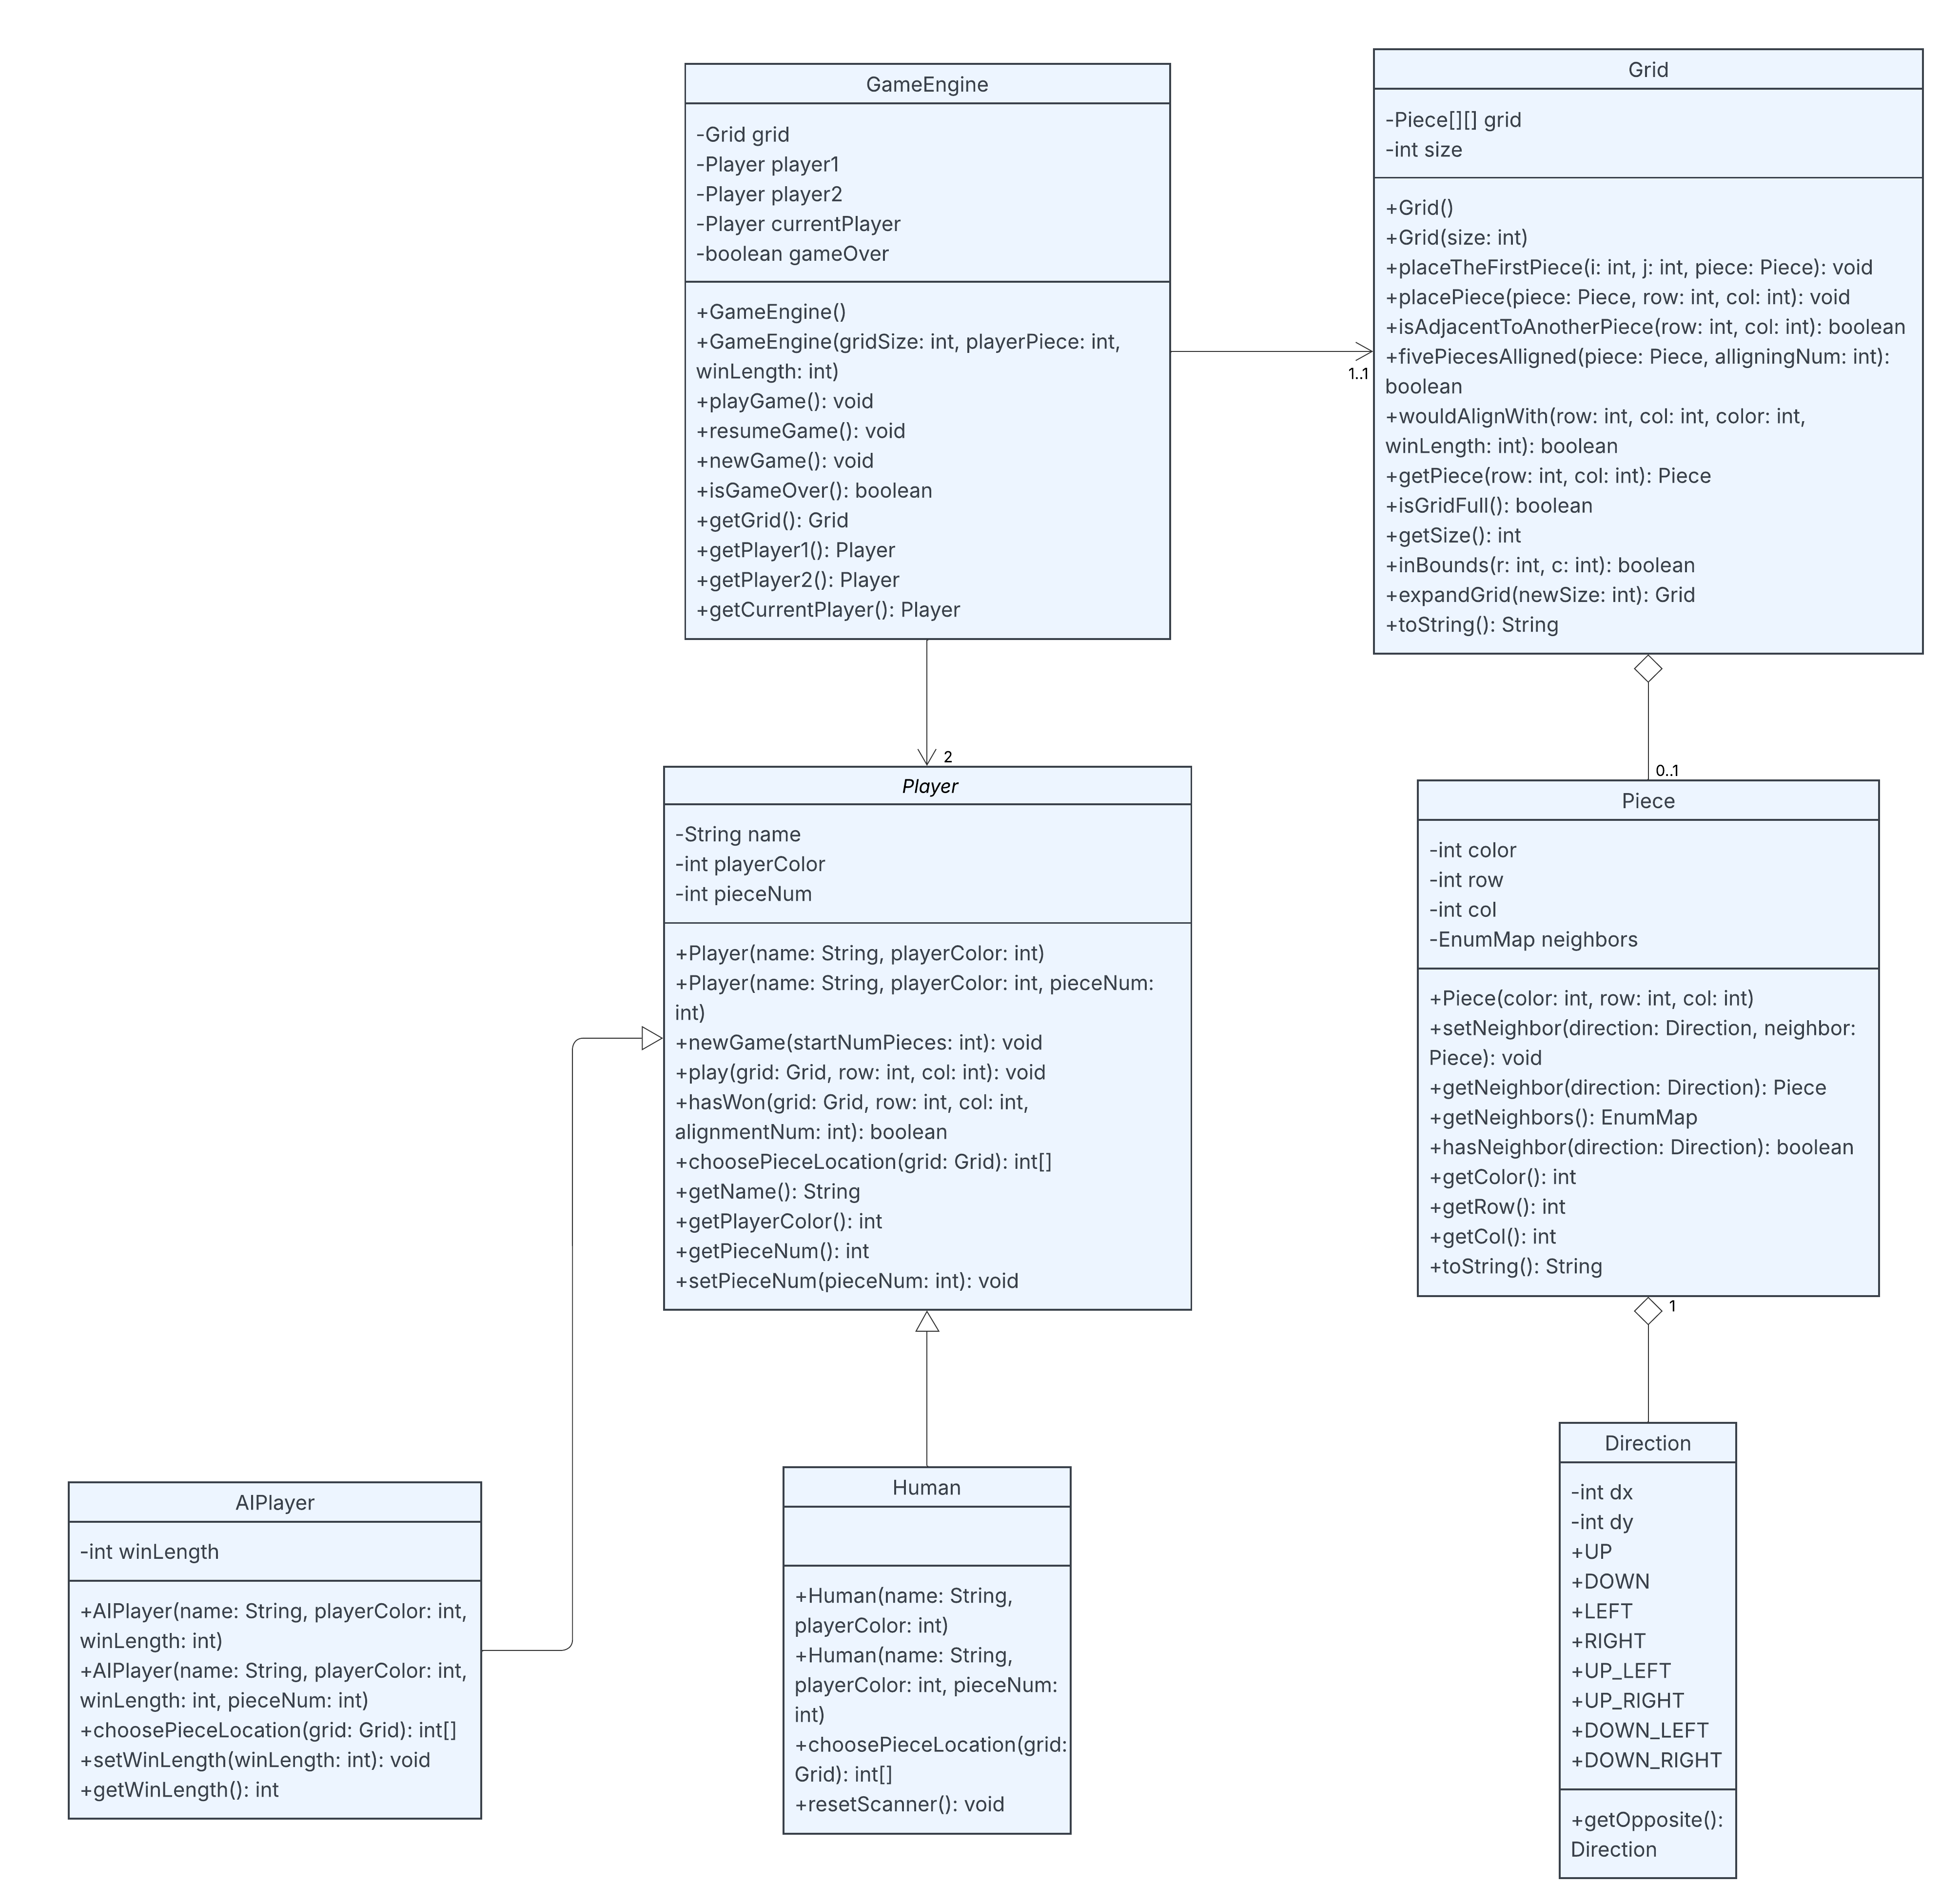
\includegraphics[width=1\textwidth]{img/gomoku-UML.png}
    \caption{Diagramme UML de la logique du projet Gomoku}
    \label{fig:uml}
\end{figure}

\end{document}
